\documentclass{beamer}
\usepackage{mathtools}
\usepackage{xspace}
\usepackage{tabu}
\usepackage{commath}

\let\arrowvec\vec
\renewcommand{\vec}[1]{\ensuremath{\mathbf{#1}}}
\newcommand{\integral}[1]{\ensuremath{\left\langle #1 \right\rangle}}
\newcommand{\closure}[1]{\ensuremath{\mathcal{E}(#1)}}
\newcommand{\T}[1]{\ensuremath{#1^\textnormal{T}}}
\newcommand{\R}{\ensuremath{\mathbb{R}}\xspace}
\newcommand{\SN}{\ensuremath{\textnormal{S}_\textnormal{N}}\xspace}
\newcommand{\PN}{\ensuremath{\textnormal{P}_\textnormal{N}}\xspace}
\newcommand{\MN}{\ensuremath{\textnormal{M}_\textnormal{N}}\xspace}

\frenchspacing

\title{\texttt{closures-2d}}
\author{C. Kristopher Garrett, Tim Shaffer}

\begin{document}
    \frame{\titlepage}

\section{Background}

    \begin{frame}{What Are Kinetic Equations?}
        \begin{columns}[t]
            \column{0.5 \textwidth}
            \begin{block}{Macroscopic}
                \begin{itemize}
                    \item $\rho(\vec{x},t)$ -- Density
                    \item $\vec{u}(\vec{x},t)$ -- Velocity
                    \item $E(\vec{x},t)$ -- Kinetic Energy
                \end{itemize}
                Discretize \vec{x}, $t$ into 100 values: 4GB memory requirement
            \end{block}
            \column{0.5 \textwidth}
            \begin{block}{Mesoscopic}
                \begin{itemize}
                    \item $f(\vec{x},\vec{v},t)$ -- Density with respect to space \emph{and velocity}
                \end{itemize}
                Discretize \vec{x}, \vec{v}, $t$ into 100 pieces: 800TB memory requirement
            \end{block}
        \end{columns}

        \vfill

        Macroscopic can be derived from mesoscopic
        \begin{itemize}
            \item $\rho(\vec{x},t) = \int_{\R^3} f \dif \vec{v}$
            \item $\vec{u}(\vec{x},t) = \frac{1}{\rho} \int_{\R^3} \vec{v}f \dif \vec{v}$
            \item $E(\vec{x},t) = \frac{1}{2} \int_{\R^3} \| \vec{v} - \vec{u} \|^2 \dif \vec{v}$
        \end{itemize}
    \end{frame}

    \begin{frame}{What Are Kinetic Equations?}
        \begin{block}{Form of Kinetic Equation -- Neutral Particles}
            $\partial_t f + \vec{v} \cdot \nabla_\vec{x} = C(f)$
        \end{block}

        \vfill

        Left side is the transport equation
        \[\alert{\partial_t f + \vec{v} \cdot \nabla_\vec{x}} = C(f)\]

        \vfill

        Right side governs collisions
        \[\partial_t f + \vec{v} \cdot \nabla_\vec{x} = \alert{C(f)}\]
        \vfill

        Collisions change the direction of particles

        The collision operator is problem dependent
    \end{frame}

    \begin{frame}{What Are Kinetic Equations?}
        First used for rarefied gas dynamics (e.g. high altitude gases where collisions do not dominate the physics)

        \[\partial_t f + \vec{v} \cdot \nabla_\vec{x} = C(f)\]
        where $\int C(f) \dif \vec{v} = 0$.

        \vfill

        Integrate against \vec{v} to get First Euler/Navier-Stokes equation
        \[\partial_t \rho + \nabla_{\vec{x}} \cdot (\rho \vec{u}) = 0\]

        \vfill

        Other areas:
        \begin{itemize}
            \item Radiation transport
            \item Plasma simulations
        \end{itemize}
    \end{frame}

\section{Theory}

    \begin{frame}{What Are Spherical Harmonics?}
        \begin{block}{(Real) Spherical Harmonics}
            \begin{equation*}
                Y_{\ell m}(\mu,\phi) =
                \begin{dcases}
                    \sqrt{2} N_\ell^{|m|} P_\ell^{|m|}(\mu) \sin(|m|\phi), & m < 0 \\
                    N_\ell^0 P_\ell(\mu), & m = 0 \\
                    \sqrt{2} N_\ell^m P_\ell^m(\mu) \cos(m\phi), & m > 0
                \end{dcases}
            \end{equation*}
            where $N_\ell^m = \sqrt{\frac{2\ell + 1}{4\pi}\frac{(\ell - m)!}{(\ell + m)!}}$.
            \begin{itemize}
                \item Spherical harmonics are an orthonormal basis of $L^2(S^d)$
                \item They are usually considered for the unit sphere $S^2$
                \item For $d = 1$, you get Fourier series
                \item For $d = 2$, you get $Y_{\ell m}(\mu,\phi)$ where $\ell$ is the degree and $m$ is the order
            \end{itemize}
        \end{block}
        \alert{steal pic}
    \end{frame}

    \begin{frame}{Kinetic Problem}
        \begin{block}{Unit Speed, Isotropic Scattering}
            \begin{equation*}
                \partial_t f + \Omega \cdot \nabla_\vec{x} = \frac{\sigma}{4\pi} \integral{f} - \sigma f
            \end{equation*}
            where $x \in \R^3$, $\Omega \in S^2$, $\sigma$ is the scattering cross section, and $\integral{\cdot} = \int_{S^2} \cdot \dif \Omega$.
        \end{block}

        \vfill

        \begin{itemize}
            \item Let $\vec{m}(\Omega) = \left(Y_{0,0}, Y_{1,-1}, Y_{1,0}, Y_{1,1}, \dots, Y_{N,-N}, \dots, Y{N,N}\right)^T$ be a vector of spherical harmonics up to and including degree $N$
            \item Take moments with respect to \vec{m}
            \item $\vec{u}(\vec{x}, t) = \integral{\vec{m}(\Omega) f(\vec{x}, \Omega, t)}$
        \end{itemize}
        \alert{Why? Because $u_{\ell m} = f_{\ell m}$ and the collision operator is diagonalized}
    \end{frame}

    \begin{frame}{Moment Closures}
        \begin{block}{Exact Moment System}
            $\partial_t \vec{u} + \nabla_x \cdot \integral{\Omega \vec{m} f} = \Dif \vec{u}$
        \end{block}

        \vfill

        System is not closed

        Think of 1D case with $\vec{m}\left(\mu) = (1, \mu, \mu^2, \dots, \mu^n\right)$:
        \begin{align*}
            \partial_t u_0 + \partial_x u_1 &= \Dif_{00} u_0 \\
            \partial_t u_1 + \partial_x u_2 &= \Dif_{11} u_1 \\
            \partial_t u_2 + \partial_x u_3 &= \Dif_{22} u_2 \\
            \vdots \\
            \partial_t u_n + \partial_x u_{n + 1} &= \Dif_{nn} u_n
        \end{align*}

        \vfill

        \alert{To close the system}: Replace $f$ with $\closure{\vec{u}}$ such that $\integral{\vec{m} \closure{\vec{u}}} = \vec{u}$
    \end{frame}

    \begin{frame}{Moment Closures}
        \begin{block}{\PN Moment Closure}
            \[ \closure{\vec{u}} = \vec{u}^T \vec{m} \]
        \end{block}
        \begin{block}{\MN Moment Closure}
            \[ \closure{\vec{u}} = \exp\left(\T{\vec{\alpha}} \vec{m}\right) \]
            where \vec{\alpha} solves $\min_{\hat{\alpha}} \integral{\exp\left(\T{\hat{\vec{\alpha}}} \vec{m}\right)} - \T{\hat{\vec{\alpha}}} \vec{u}$
        \end{block}

        \vfill

        \alert{Two notes}
        \begin{itemize}
            \item The moment closure occurs on every spatial cell and every time point
            \item All the moment closures are \textbf{independent}
        \end{itemize}
    \end{frame}

    \begin{frame}{Discrete Ordinates (\SN)}
        \begin{itemize}
            \item Textbook method used in many applications
            \item Simple, direct approximation of the kinetic equation using quadrature sets on the unit sphere
            \item Strong ray effects at low orders
        \end{itemize}

        \vfill

        \begin{equation*}
            \partial_t f_q + \Omega_q \cdot \nabla_x f_q = \frac{\sigma}{4\pi} \sum_{q' = 1}^Q w_{q'} f_{q'} - \sigma f_q
        \end{equation*}
        where $f_q(x,t) \approx f(x,\Omega_q,t)$ for $q = 1, \dots, Q$
    \end{frame}

\section{Implementation}

    \begin{frame}{Initial Conditions}
        \begin{block}{Gaussian Initial Condition}
            Two dimensional Gaussian function centered at the origin

            \begin{equation*}
                f(x, y, \Omega, t=0) = \max \left( \frac{1}{2 \pi \sigma_g^2} e^{-(x^2 + y^2) / (2 \sigma_g^2)}, \texttt{floor} \right), 
            \end{equation*}
            where $\sigma_g$ is the configurable Gaussian sigma and \texttt{floor} is the floor value for the grid.
        \end{block}

        \vfill

        \begin{block}{Delta Initial Condition}
            Limiting case of Gaussian I.C. with $\sigma_g \to 0$.

            Simulates an initial pulse of particles distributed isotropically along an infinite line in space.

            Centermost cell is given a high initial density.
        \end{block}
    \end{frame}

    \begin{frame}{Initial Conditions}
        \begin{block}{Lattice Initial Condition}
            Checker board pattern of highly scattering and highly absorbing regions with empty initial grid.

            Reminiscent of a small section of a nuclear reactor core.
        \end{block}

        \vfill

        \begin{block}{Smooth Initial Condition}
            Primarily intended for testing convergence

            Initialize the grid points with a periodic boundary given by
            \begin{equation*}
                f(x,y,\Omega,t=0) = 1 + \sin(2\pi x)\cos(2\pi y).
            \end{equation*}
        \end{block}
    \end{frame}

    \begin{frame}{Initial Conditions}
        \begin{columns}
            \column{0.33 \textwidth}
            \centering
            Gaussian Initial Condition

            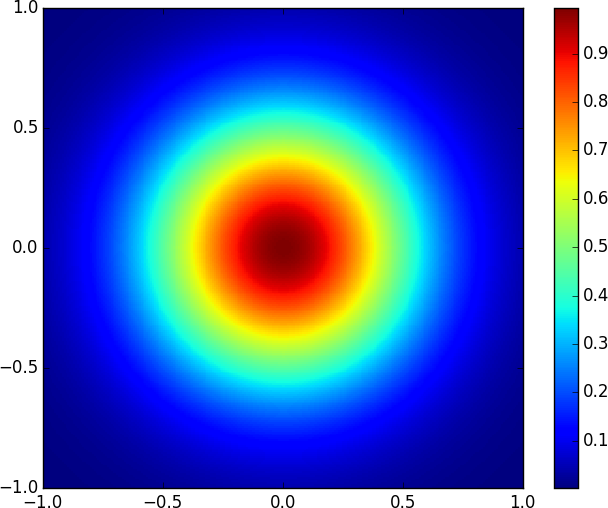
\includegraphics[width=\textwidth]{initcond_gaussian.png}

            \column{0.33 \textwidth}
            \centering
            $\sigma_T$ for Lattice Initial Condition

            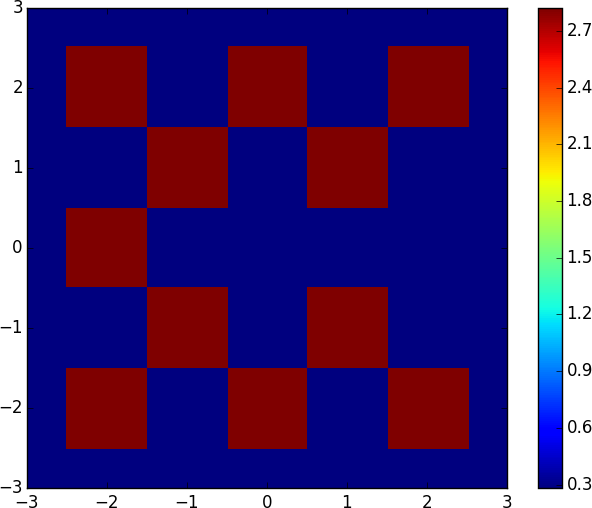
\includegraphics[width=\textwidth]{initcond_lattice-t.png}

            \column{0.33 \textwidth}
            \centering
            Smooth Initial Condition

            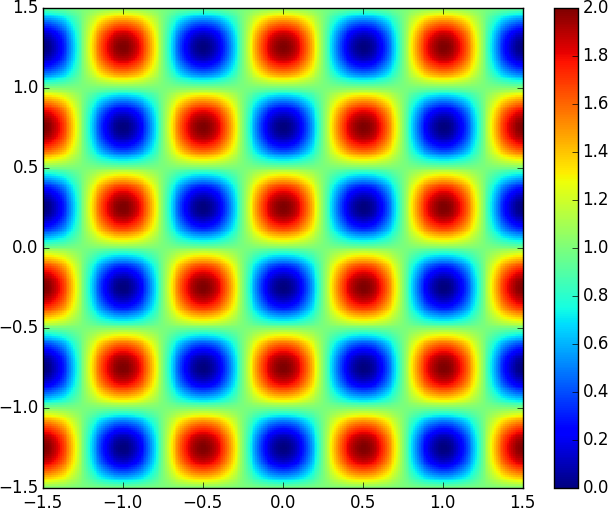
\includegraphics[width=\textwidth]{initcond_smooth.png}
        \end{columns}
    \end{frame}

    \begin{frame}{Implementation Notes}
        \begin{columns}
            \column{0.5 \textwidth}
            Spherical Harmonics: $Y_{\ell m}(\Omega)$
            \begin{itemize}
                \item $\ell = 0, \dots, N$ is the degree
                \item $m = -\ell , \dots, \ell$ is the order
                \item Total number of moments: $M = (N + 1)^2$
            \end{itemize}

            \column{0.5 \textwidth}
            \begin{tabu}{X[$] X[$] X[$] X[$] X[$]}
                         &          & Y_{0,0} &         &         \\
                         & Y_{1,-1} & Y_{1,0} & Y_{1,1} &         \\
                Y_{2,-2} & Y_{2,-1} & Y_{2,0} & Y_{2,1} & Y_{2,2}
            \end{tabu}
        \end{columns}

        \vfill

        Quadrature in angle: $\Omega_q, w_q$
        \begin{itemize}
            \item $\int_{S^2} F(\Omega) \dif \Omega \approx \sum_q w_q F(\Omega_q)$
            \item Product quadrature: $\int_{S^2} \dif \Omega = \int_{-1}^1 \int_0^{2\pi} \dif \phi \dif \mu$
            \item $n_g$ Gaussian nodes on $\mu$ axis
            \item $2n_g$ equally spaced nodes on latitudinal circles (for $\phi$)
            \item Total number of quadrature points $Q = 2n_g^2$
            \item Integrates spherical harmonics of degree $2n_g - 1$ exactly!
        \end{itemize}
    \end{frame}

    \begin{frame}{Spatial Discretization}
        \begin{itemize}
            \item Use a 2D Cartesian mesh with constant cell size to break problem space into an $m$ x $n$ grid
            \item Store density with respect to direction for each cell
            \item Also need a halo of ghost cells for boundary conditions, MPI communication
        \end{itemize}

        \vfill

        \begin{block}{Upwinding}
            Since $f$ depends on position, \textbf{direction}, and time, we \emph{must} use information from the correct side

            \alert{steal pictures?}
        \end{block}
    \end{frame}

    \begin{frame}{Time Stepping}
        \begin{block}{CFL Condition}
            A small enough time step is necessary for convergence. In this case,
            \begin{equation*}
                \frac{\Delta t}{\Delta x} + \frac{\Delta t}{\Delta y} \leq 1
            \end{equation*}
        \end{block}

        \vfill

        \begin{block}{Heun's Method}
            To compute a first estimate, carry out two Euler steps.
            Now use the average of the initial state and the estimate.
            \begin{itemize}
                \item Explicit, two-stage Runge-Kutta method
                \item Second order accurate
                \item Strong stability preserving
            \end{itemize}
        \end{block}
    \end{frame}

    \begin{frame}{Results}
        Tabulate some runtimes, convergence rates, etc.
    \end{frame}

    \begin{frame}
        Show some plots
    \end{frame}

\section{Software}
    \begin{frame}{Release}
        We are releasing this code as open source software.

        \vfill

        Built using SCons

        \vfill

        Depends on
        \begin{itemize}
            \item GSL
            \item BLAS
            \item LAPACK
            \item OpenMP (optional, provided by many compilers)
            \item Open MPI (optional)
        \end{itemize}
    \end{frame}

    \begin{frame}{Tests}
        We implemented automated testing for the following aspects. The testing code carries out
        \begin{itemize}
            \item Regression tests -- compare output to reference data included with the software
            \item Convergence tests -- measure the effect of decreasing the cell size on the precision of the output
            \item Mass Conservation tests -- check that total density remains the same
        \end{itemize}

        \vfill

        The testing code is written in Python and integrated with the build system
    \end{frame}

    \begin{frame}{Improvements}
        Algorithmic changes:
        \begin{itemize}
            \item Added experimental Lebedev quadrature
            \item Removed $\delta$ factor for ansatz correction in \texttt{momopt}
            \item Changed \texttt{momopt}'s regularization in case of bad condition number
        \end{itemize}

        \vfill

        Software-related improvements:
        \begin{itemize}
            \item Cross-platform build system
            \item Automated testing
            \item Better MPI communication
            \item Improved documentation
            \item Improved interface
            \item Bugfixes
            \item Profiling and optimization
        \end{itemize}
    \end{frame}

    \begin{frame}{Bibliography}
        cite that presentation, linesource paper
    \end{frame}
\end{document}
